%---------------------------------------------------------------------------------
\chapter{Numerical methods}
\label{chap:numerical-methods}
%---------------------------------------------------------------------------------
\section{Ordinary differential equation}
An ordinary differential equation (ODE) is an equation that contains derivatives of single independent variable functions. Examples of ODEs would be $\frac{df}{dx}=-x$ and $\frac{df}{dx} + \frac{dg}{dx} = 4x$, where $x$ is an independent variable, $f$ and $g$ are functions of $x$. In general, ODEs are used to describe changes. One of the simplest example is speed, change in distance travelled per unit time. 

There are different ways to describe an ODE. The order of an ODE is the order of the highest derivative in an ODE. The ODE $\frac{d^3f}{dx^3} = -1$ has order 3. Other than the order, ODEs can be classified into linear or non-linear ODE. Linear ODEs are functions that can be expressed as linear combinations of derivatives, while non-linear ODEs cannot. The equation, $\frac{df}{dx} \frac{dg}{dx} = 1$, for example, is non-linear ODE; the equation $\frac{df}{dx} + \frac{dg}{dx} = 1$ is linear. Linear ODE can further be categorised into homogeneous and non-homogeneous ODEs. In a general linear ODE, $a_0(x)f(x)+a_1(x)f'(x)+...+a_n(x)f^{(n)}(x)+b(x) = 0$, the function is homogeneous if $b(x) = 0$ and non-homogeneous if $b(x) \neq 0$.

ODEs are widely used in biological problem. An example of biological problem would be the SEIR model. The SEIR model describes the spread of a disease in a population with time $t$. The model compartmentalises the population into groups of susceptibles ($S$), exposed ($E$), infectious ($I$) and recovered ($R$). Transitions of individuals from groups are described by a system of ODEs, with independent variable time $t$. It is defined as 
\begin{align}
\label{eqn:SEIR-model}
    \frac{dS(t)}{dt} &= -\beta S(t)I(t),  \\ 
    \frac{dE(t)}{dt} &= \beta S(t)I(t) - \kappa E(t), \\
    \frac{dI(t)}{dt} &= \kappa E(t) - \gamma I(t), \\
    \frac{dR(t)}{dt} &= \gamma I(t) \label{eqn:SEIR-end}
\end{align}
where the parameters $\beta$, $\kappa$ and $\gamma$ are infection rate, incubation rate and recovery rate respectively. The incidence cases, $N$ at time, $t$, is defined as the difference between the current total number of infected and recovered and that of the previous time, according to the equation
\begin{equation}
    N(t) = I(t) + R(t) - I(t-1) - R(t-1)
\end{equation}
Figure \ref{fig:SEIR_simulation} shows the incidence cases simulated by the SEIR model.

\begin{figure}
    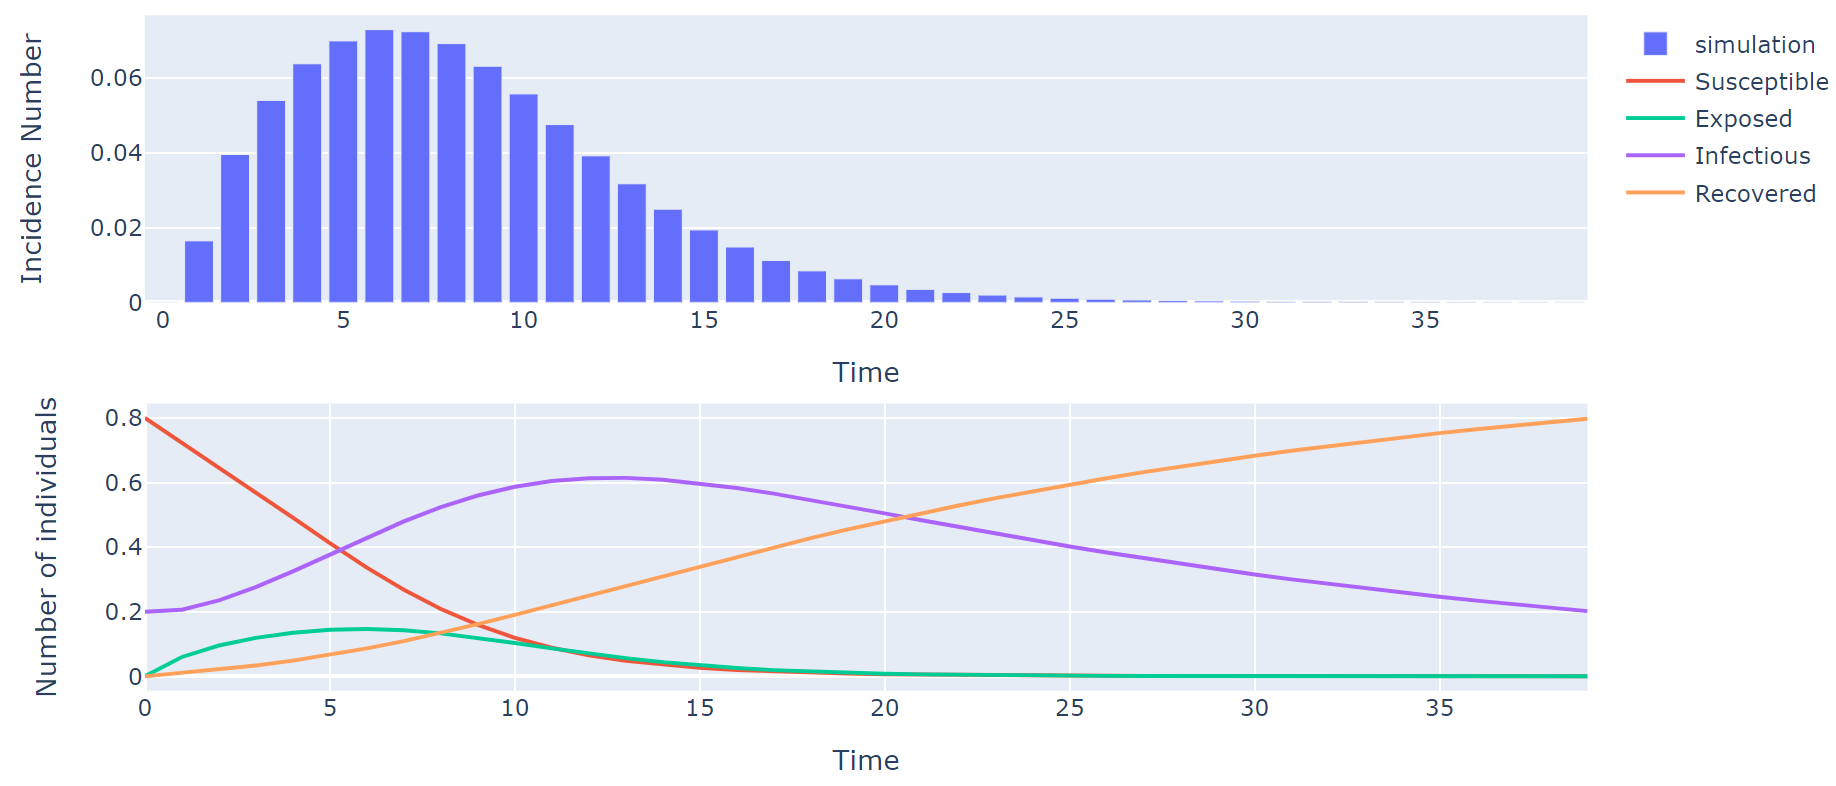
\includegraphics[width=0.95\columnwidth]{SEIR_simulation}
    \caption{Simulation of the SEIR model. The bar graph shows the incidence number, while the line graph shows the number of individuals in each group. All values shown are in fractions of the whole population.}
    \label{fig:SEIR_simulation}
\end{figure}

Another example is the modelling of excitable systems. The heart muscle cells and nerve cells are excitable systems. The Hodgkin \& Huxley model models the ionic currents across the cell membrane, to explain the action potential of nerve cells\cite{Keener2009}.
Their model is defined as
\begin{equation}
\label{model:HH}
    C_m \frac{dV}{dt} = -g_{\text{eff}}(V - V_{\text{eq}}) + I_{\text{app}} \\
\end{equation}
where $C_m$ is membrane capacitance, $V$ is membrane potential, $g_{\text{eff}}$ is sum of conductance for all ion channels, $V_{\text{eq}}$ is membrane resting potential and $I_{\text{app}}$ is applied current. Here, the independent variable is also time $t$. The value of potential is obtained by subtracting the membrane resting potential from the membrane potential, that is $V - V_{\text{eq}}$. Figure \ref{fig:AP_simulation} shows the simulated action potential of the Hodgkin and Huxley model. 

\begin{figure}
\centering
    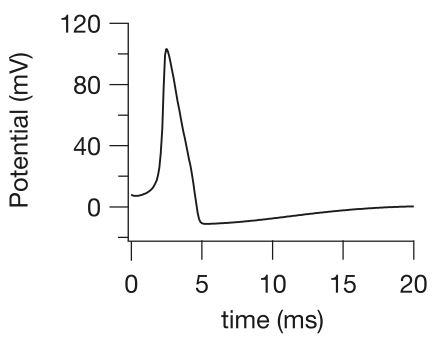
\includegraphics[width=0.5\columnwidth]{AP_simulation}
    \caption{The action potential in the Hodgkin and Huxley model, adapted from \cite{Keener2009}.}
    \label{fig:AP_simulation}
\end{figure}

\section{Initial value problem}
Given an ODE system, we would like to solve for the function. As an example, given an ODE $\frac{df(x)}{dx} = -f(x)$, we would like to know the function $f$. To solve ODE systems, initial conditions are required to pinpoint the solution of interest, as there are infinitely possible solutions to an ODE. The ODEs, together with the initial conditions, set up the initial value problem.

A general form of an initial value problem is as follows: 
\begin{align}
\label{eqn:initial_value_start}
    y'&=f(x,y)\\
    y(x_0) &= y_0 \label{eqn:initial_value}
\end{align}
for $x \in [x_0, X_M]$, where Eq.~\eqref{eqn:initial_value} describes the initial condition. For example, initial values of $S(0)=0.8, E(0)=0, I(0)=0.1$ and $R(0)=0$ are used to solve the SEIR model in Figure \ref{fig:SEIR_simulation}.

\section{Numerical method}
Many ODE systems cannot be solved analytically. Some examples would be the given SEIR Model, Eqs.~\eqref{eqn:SEIR-model}-\eqref{eqn:SEIR-end} and Hodgkin \& Huxley Model, Eq.~\eqref{model:HH}. Solutions to such models have to be estimated by numerical methods.

Throughout the report, the following notation will be used:
\begin{itemize}
    \item $y_n$ - numerical approximation of $y(x_n)$
    \item $y(x_n)$ - analytical solution at mesh point $x_n$
    \item $x_n$ - mesh points of defined range, where
        \begin{align}
            x_n &= x_0 + nh\\
            h &= \frac{(X_M - x_0)}{N}
        \end{align}
        for $n = 0,\dots, N$
    \item $h$ - step size
\end{itemize}

\subsection{One-step methods}
\label{subsec:one-step-method}
The simplest numerical method in solving ODEs is Euler's explicit method. Intuitively, Euler's explicit method assumes for a small step size $h$, the solution of the function can be estimated by its tangent line. As seen in Figure \ref{fig:Euler_method}, following the tangent line at point $x_0$, the difference between the $y$ value for point $x_0$ and point $x_1$ is $hF(x_0,y_0)$. So, the estimated value of $y_1$ is $y_0 + hF(x_0,y_0)$, where $y_0$ is the value of solution curve at $x_0$.

\begin{figure}
\centering
    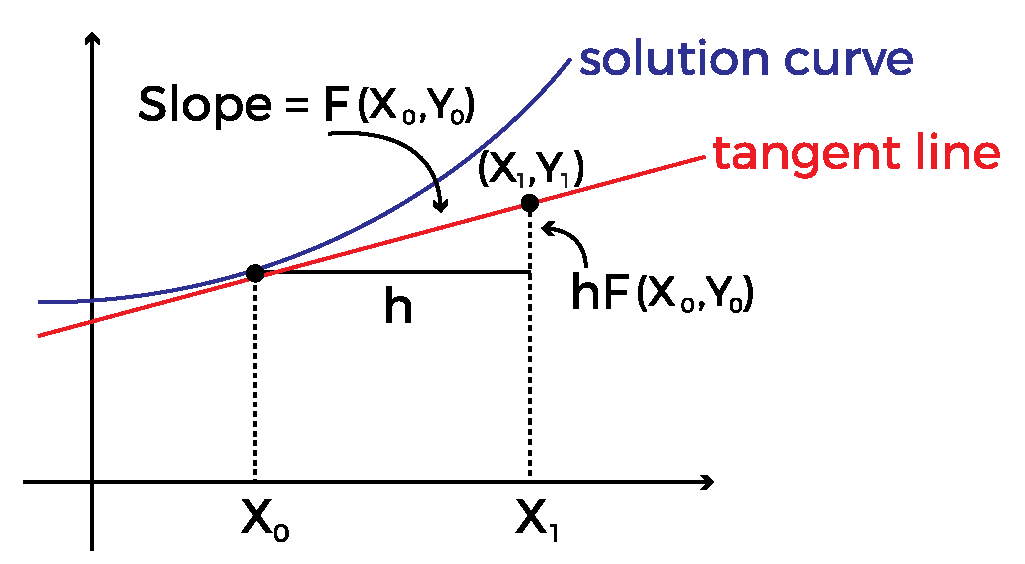
\includegraphics[width=0.5\columnwidth]{Euler_method_img}
    \caption{Intuition of Euler's method, adapted from \cite{CalcWorkshop2019}.}
    \label{fig:Euler_method}
\end{figure}

Euler's explicit method has the following definition,  
\begin{equation}
    y_{n+1} = y_n + hf(x_n,y_n)\\
\end{equation}
Starting from the initial value, the solution at the subsequent mesh point is estimated to follow a straight line with gradient as given.

The implementation is as follows:

\begin{algorithm}[H]
    \SetAlgoLined
    \SetKwInOut{Output}{Output}
    \Output{mesh points and its numerical solution}
    solution = [initial value]\;
    meshpoints = [starting point]\;
    \For{$n$ \text{from} 1 \text{to total number of mesh points}}{
    solution.append(solution[$n-1$] + step size $\times$ $f$(meshpoints[$n-1$], solution[$n-1$])\;
    meshpoints.append(meshpoints[$n-1$] + $n$ $\times$ step size)\;
    }
    \Return{meshpoints and solution}\;
\caption{Euler's explicit method}
\end{algorithm}

A vector containing the numerical solution and a vector of mesh points are initialised with their respective initial values. At each iteration, the mesh point and the numerical solution at the mesh point are calculated. The series of mesh points and its solution are returned. The mesh points are returned for consistency of the software, where all methods return the same outputs. Adaptive methods does not have fixed step sizes, thus it is important to return the mesh points. 

Truncation error of the numerical methods is defined to be the difference between the exact solution and the numerical solution, assuming the exact solution at the previous mesh point is known. We have that the truncation error for Euler's explicit method is

\begin{equation}
\label{eqn:trun_err_def}
    T_n \defeq \frac{y(x_{n+1}) - y(x_{n})}{h} - f(x_n, y(x_n))
\end{equation}
According to Taylor's series expansion, we have 
\begin{equation}
\label{eqn:Taylor_expansion}
    y(x_n + h) = y(x_n) + hy'(x_n) + \frac{1}{2}hy''(\xi_n)
\end{equation}
for some $\xi_n \in (x_n, x_{n+1})$. Substitute (\ref{eqn:Taylor_expansion}) to (\ref{eqn:trun_err_def}), noting that $f(x_n, y(x_n)) = y'(x_n)$, we get
\begin{equation}
    T_n = \frac{1}{2}hy''(\xi_n)
\end{equation}
Therefore, the truncation error for Euler's explicit method varies linearly with the step size.

A test problem
\begin{align}
\label{eqn:example_model}
    f(x,y) &= -y \\
    y(0) &= 1 \label{eqn:example-end}
\end{align}
for $x \in [0, 5]$ is used throughout this report to check that the implementation is in line with the theory. The analytical solution to this problem is $y = e^{-x}$. Some examples of solutions to the given test problem Eqs.~\eqref{eqn:example_model}-\eqref{eqn:example-end} can be found via this link: \href{https://nbviewer.jupyter.org/github/FarmHJ/numerical-solver/blob/main/examples/solver_convergence.ipynb}{\underline{\emph{test problem notebook}}}. This Jupyter Notebook is a tutorial example that demonstrates the use of the fully tested package I developed on the test problem.

With the test problem Eqs.~\eqref{eqn:example_model}-\eqref{eqn:example-end} as a reference, the truncation error versus step size graph is shown in Figure \ref{fig:Euler_explicit_error_behaviour}. The computation and comparison of one-step methods and their truncation error can be found at this link: \href{https://nbviewer.jupyter.org/github/FarmHJ/numerical-solver/blob/main/examples/Onestep_methods_convergence.ipynb}{\underline{\emph{error behaviour of one-step methods}}}. The truncation error is computed by taking the difference between the exact solution and the numerical solution at a randomly chosen $x$ value of 3. The truncation error is computed for solutions obtained by using different step sizes. Figure \ref{fig:Euler_explicit_error_behaviour} is plotted in logarithmic scale for both variables. It can be observed that $\log |T_n|$ increases linearly with $\log h$. The line gradient of 1 shows that $|T_n| \propto h$, which matches the theoretical prediction. 

\begin{figure}
    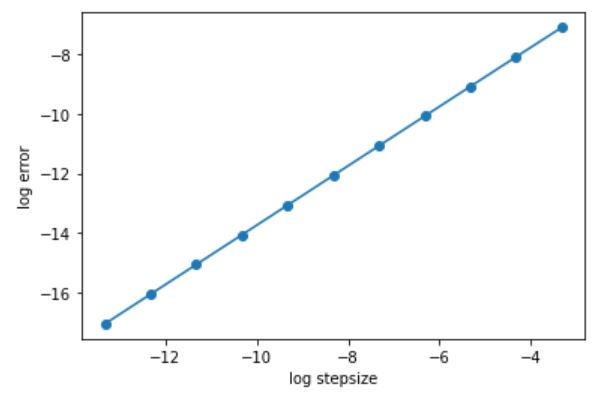
\includegraphics[width=0.95\columnwidth]{Euler_explicit_error_behaviour}
    \caption{Truncation error of Euler's explicit method for various step sizes. The test problem Eqs.~\eqref{eqn:example_model}-\eqref{eqn:example-end} is solved with Euler's explicit method at different step sizes. The error is the absolute difference between exact solution and numerical solution at $x=3$.}
    \label{fig:Euler_explicit_error_behaviour}
\end{figure}

Other than Euler's explicit method, the other one-step methods implemented are Euler's implicit method, the trapezium rule method and the four-stage explicit Runge-Kutta method. Euler's implicit method is defined to be
\begin{equation}
    y_{n+1} = y_n + hf(x_{n+1},y_{n+1}),\\
\end{equation}
while the trapezium rule method is
\begin{equation}
    y_{n+1} = y_n + \frac{1}{2}h[f(x_n,y_n) + f(x_{n+1},y_{n+1})].\\
\end{equation}
The definition of the four-stage Runge-Kutta method is
\begin{equation}
    y_{n+1} = y_n + \frac{1}{6}h(k_1 + 2k_2 + 2k_3 + k4)
\end{equation}
where
\begin{align}
    k_1 &= f(x_n, y_n) \\
    k_2 &= f(x_n + \frac{1}{2}h, y_n + \frac{1}{2}hk_1) \\
    k_3 &= f(x_n + \frac{1}{2}h, y_n + \frac{1}{2}hk_2) \\
    k_4 &= f(x_n + h, y_n + hk_3).
\end{align}

Using the same definition for truncation error as in Eq.~\eqref{eqn:trun_err_def}, we have that the truncation error of Euler's implicit method, the trapezium rule method and the four-stage Runge-Kutta method are $T_n = -\frac{1}{2}hy''(\xi_n)$ for $\xi_n \in (x_n, x_{n+1})$, $T_n = -\frac{1}{12}h^2y^{(3)}(\xi_n)$ for $\xi_n \in (x_n, x_{n+1})$ and $T_n = \mathcal{O}(h^4)$ respectively.

These methods are tested on the test problem Eqs.~\eqref{eqn:example_model}-\eqref{eqn:example-end}, and the truncation error behaviour graph is shown in Figure \ref{fig:onestep_error_behaviour}. Since the graph is plotted in logarithmic scale, the gradient of the lines shows the order of accuracy of the methods. The gradient for Euler's explicit, Euler's implicit, the trapezium rule method and the four-stage Runge-Kutta method are 1, 1, 2 and 4 respectively. The gradients on the graph match the theoretical behaviour of truncation error. In Figure \ref{fig:onestep_error_behaviour}, the truncation error behaviour of Euler's implicit method overlaps that of Euler's explicit method because both have the same order of accuracy. 

\begin{figure}
    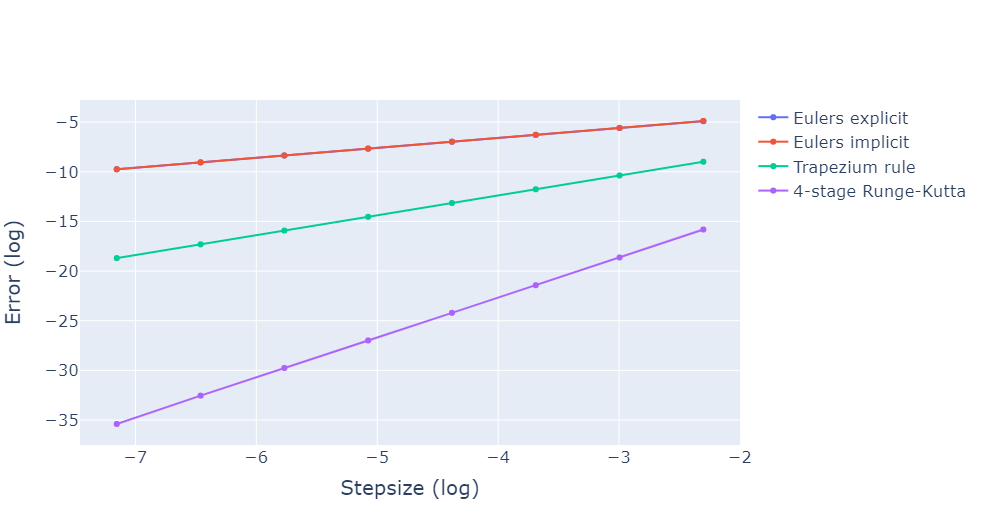
\includegraphics[width=0.95\columnwidth]{onestep_error_behaviour}
    \caption{Truncation error of Euler's explicit method, Euler's implicit method, the trapezium rule method and the four-stage Runge-Kutta method for various step sizes. The test problem Eqs.~\eqref{eqn:example_model}-\eqref{eqn:example-end} is solved with Euler's explicit method, Euler's implicit method, the trapezium rule method and the four-stage Runge-Kutta method at different step sizes. The error is the absolute difference between exact solution and numerical solution at $x=3$. The line for Euler's implicit method overlaps the line for Euler's explicit method because both have the same order of accuracy. The truncation errors follow theoretical prediction.}
    \label{fig:onestep_error_behaviour}
\end{figure}

\subsection{Predictor-corrector methods}
\label{sec:predictor-corrector}
For implicit one-step methods, the fixed point iteration algorithm is used to obtain the numerical solution. Implicit functions cannot be solved with a general method, therefore a general algorithm, the fixed point iteration, is used to estimate the solution to the implicit functions. Initial guesses for this algorithm are taken as the numerical solution at previous mesh point. However, in practice, the computational cost of the fixed point algorithm is too high. The predictor-corrector method suggests a more carefully chosen initial guess for the implicit methods. An explicit numerical method is used as a predictor for the initial guess of an implicit method. The initial guess is then used for the iterations in the algorithm to solve an implicit function. The implicit method that refines the solution is known as the corrector method. 

The Euler-Trapezoidal method is a predictor-corrector method that uses Euler's explicit method as the predictor and the trapezium rule method as the corrector. In this implementation, the trapezium rule method corrector is iterated until a set of conditions are satisfied. The conditions are set to be the difference between the current iteration and the previous iteration is lesser than a given threshold value or the number of iterations exceeds a certain amount. Figure \ref{fig:predictor_corrector_error_behaviour} shows the graph of $\log |T_n|$ against $\log h$ for the Euler-Trapezoidal method.

\begin{figure}
    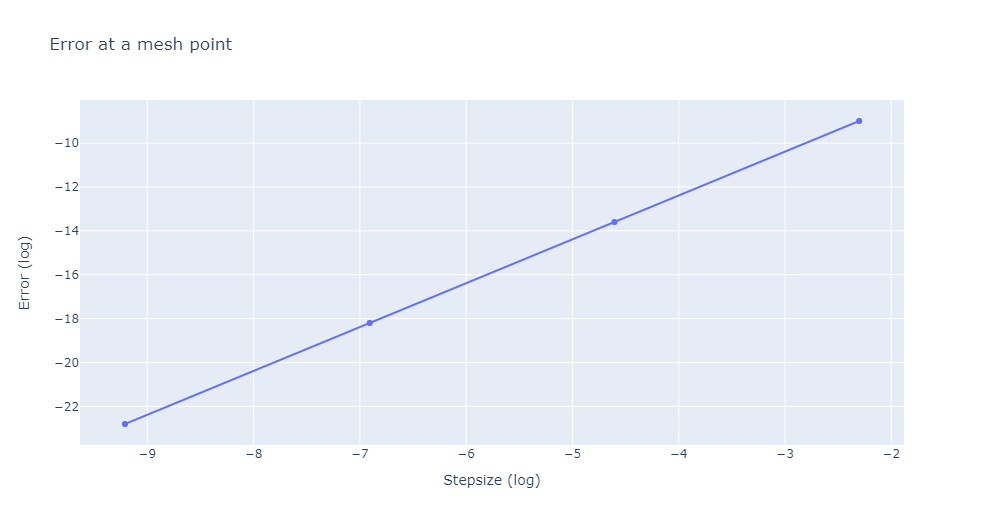
\includegraphics[width=0.95\columnwidth]{predictor_corrector_error_behaviour}
    \caption{Error of Euler-Trapezoidal method for various step sizes. The test problem Eqs.~\eqref{eqn:example_model}-\eqref{eqn:example-end} is solved with Euler-Trapezoidal method at different step sizes. The error is the absolute difference between exact solution and numerical solution at $x=3$.}
    \label{fig:predictor_corrector_error_behaviour}
\end{figure}

\subsection{Adaptive method}
\label{sec:adaptive-method}
In some types of problem, the solution to the problem exhibits a behaviour where step sizes have to be sufficiently small to obtain a stable solution. In other words, the solution changes rapidly as a function of the independent variable in some regions of the solution domain. Such problems are called stiff problems. In order to obtain a stable solution for stiff problems, the computational cost would be high. Moreover, such a stable solution would have resolution higher than required for practical purposes in some regions.

Adaptive methods try to achieve the desired accuracy with low computational cost. The main idea of an adaptive method is to control the precision at each mesh point and from there assumes the precision of the solution is within the desired range. To achieve this, the error at each mesh point is estimated. If the error is larger than a threshold value, a smaller step size is chosen. These steps are repeated until the error is smaller than the given threshold value.

The adaptive methods implemented in my package are based on the BS23 (Bogacki and Shampine) and RKF45 (Runge-Kutta-Fehlberg) method. A lower order method is used to estimate the solution, while a higher order method is used to estimate the error. 

Absolute tolerance and relative tolerance are used in the implementation of the adaptive methods to control the error. Similarly, the implemented adaptive method is used to solve the test problem Eqs.~\eqref{eqn:example_model}-\eqref{eqn:example-end} and tested for convergence. Two comparisons were made, one based on absolute tolerance and the other on relative tolerance. As shown in Figure \ref{fig:ode45_absolute_sum_error_behaviour} and Figure \ref{fig:ode45_relative_sum_error_behaviour}, the error of the method is smaller for smaller tolerance, regardless of absolute tolerance or relative tolerance.

\begin{figure}
    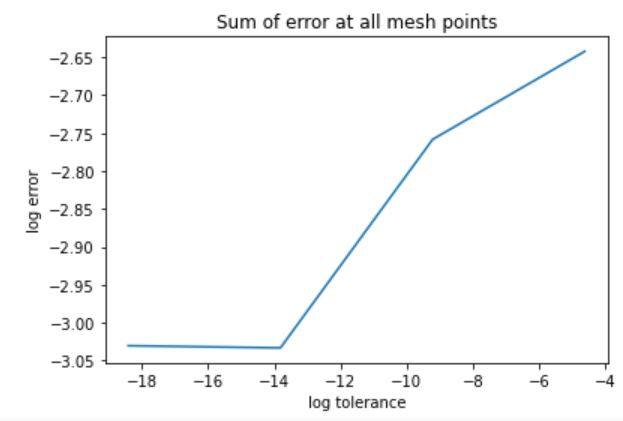
\includegraphics[width=0.95\columnwidth]{ode45_absolute_sum_error_behaviour}
    \caption{Total error of RKF45 method for various absolute tolerance values. The test problem Eqs.~\eqref{eqn:example_model}-\eqref{eqn:example-end} is solved with RKF45 method at different absolute tolerance values. The relative tolerance is fixed at $1^{-15}$. The error is the sum of absolute difference between exact solution and numerical solution at all mesh points.}
    \label{fig:ode45_absolute_sum_error_behaviour}
\end{figure}

\begin{figure}
    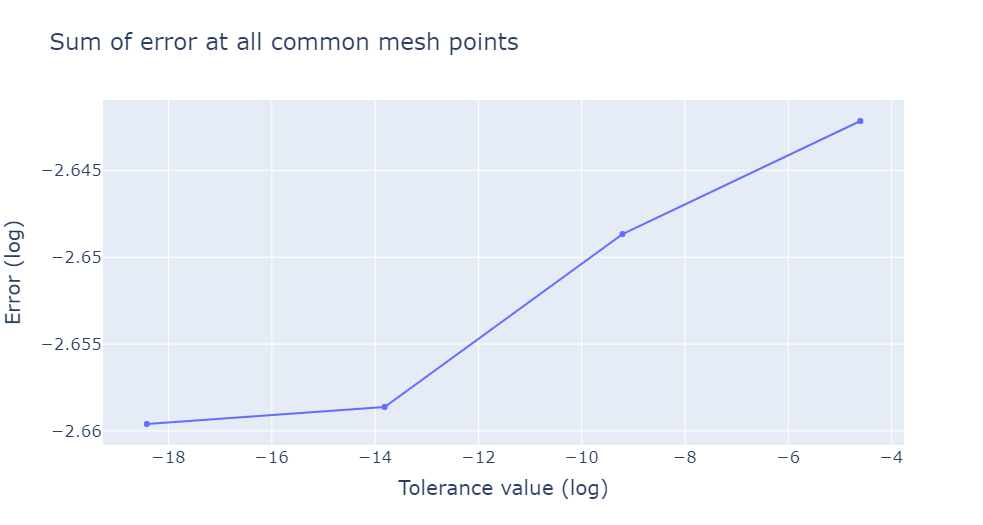
\includegraphics[width=0.95\columnwidth]{ode45_relative_sum_error_behaviour}
    \caption{Total error of RKF45 method for various relative tolerance values. The test problem Eqs.~\eqref{eqn:example_model}-\eqref{eqn:example-end} is solved with RKF45 method at different relative tolerance values. The absolute tolerance is fixed at $1^{-15}$. The error is the sum of absolute difference between exact solution and numerical solution at all mesh points.}
    \label{fig:ode45_relative_sum_error_behaviour}
\end{figure}